% pdfLaTeX
% This template was made based on the template Word file distributed by NAIST, 
% and made to be visually as similar as possible to the original template.
% For this reason the space lengths and layouts are set manually by directly indicating them.
% The font in the original Word file is Times New Roman,
% whereas the PDF output seems to be written in Computer Modern.
% This file uses LaTeX's default Computer Modern,
% but users may probably specify another font,
% since there is no specification by the format.

\documentclass[a4paper, total={14.5cm, 20.5cm}, 12pt]{article}

\usepackage{naist}

%%%%% TITLE PAGES SETTING %%%%%
\title{Theoretical Studies on Low-Speed Calculation Algorithms of $\pi$ Utilizing the Sun and the Moon} % Write your title
\author{Hanako Sentan} % Write your full name
\date{\today} % Change this to the appropriate submission date
\thesistype{Master's Thesis} % or Doctoral Dissertation
\program{Information Science and Engineering}
% or also:
% Biological Science,
% Materials Science and Engineering, 
% Data Science,
% Bionanotechnology,
% Intelligent Cyber-Physical Systems,
% Computational Biology
\supervisor{XXX} % Write your supervisor's name here.
% Change naist.sty if you want to change the title (Prof. by default)
\laboratory{xxx} % Write your lab's name here
\division{Information Science} % or Biological Science, Materials Science
\degree{Master of Engineering} % or Science, Biological Science
\keywords{$\pi$, astronomy, mathematics, computer, algorithm} % Write your thesis's keywords
%%%%% END OF THE TITLE PAGES SETTING %%%%%

\begin{document}

\maketitle
\makefrontpage
\pagenumbering{roman}
\makeabstractpage
The calculation of $\pi$ has been paid much attention since human beings appeared on the earth.

This thesis presents novel low-speed algorithms to calculate $\pi$ utilizing the sun and the moon.

This is a sample abstract. This is a sample abstract. This is a sample abstract. This is a sample abstract. This is a sample abstract. This is a sample abstract. This is a sample abstract. This is a sample abstract. This is a sample abstract. This is a sample abstract.

This is a sample abstract. This is a sample abstract. This is a sample abstract. This is a sample abstract. This is a sample abstract. This is a sample abstract. This is a sample abstract. This is a sample abstract. This is a sample abstract. This is a sample abstract.
\makekeywords
\clearpage

\tableofcontents
\listoffigures
\listoftables
\clearpage

% Contents
\pagenumbering{arabic}
\section{Introduction}
This document is a model and instructions for English dissertation.
\section{Prepare your dissertation}
Here, we will explain what you need to do when writing a dissertation.

\subsection{Structure of dissertation}
The submitted dissertation must meet the following items.

\begin{enumerate}
    \item Title
    \item Author's name
    \item Affiliation (Program)
    \item Abstract
    \item Keywords (4-5 words)
    \item Thesis committee
    \item Text (including ``introduction'' and ``conclusion'')
    \item Acknowledgements (if necessary)
    \item Reference
    \item Publication list (if necessary)
    \item Appendix (if necessary)
    \item All figures, photographs, tables, and their captions
\end{enumerate}

\subsection{Abstract and Keyword}

Make an English abstract and English keywords. In addition, the title, author, thesis committee, and affiliation are shown.

\subsection{Page layout}
The page layout is shown in Fig. \ref{fig:layout}.
The top, bottom, left, and right margins are
0.5 cm, 0.5 cm, 0.6 cm, and 0.6 cm, respectively.
The height and width of the textbody are 20.5 cm and 14.5 cm, respectively.
The font size is 12 pt. The line spacing is 1.2×.

\begin{figure}[t]
    \centering
    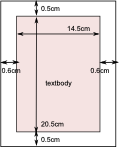
\includegraphics{src/Picture1.png}
    \caption{Page layout.}
    \label{fig:layout}
\end{figure}

\subsection{Figures, pictures, and tables}

\begin{enumerate}
    \item Use the figures, photographs, and tables originally created by the author. m in the figure in the text, indicate the corresponding English term in parentheses after the Japanese term if necessary.
    \item Insert figures, photographs, and tables together with their Japanese and English titles at appropriate positions in the text.
    \item If there are characters in the figure or photo, create them so that they can be identified by the size at the time of printing.
\end{enumerate}

The examples of figure and table are shown in Fig. \ref{fig:abyssinian} and Table \ref{tab:table}.

\begin{table}[t]
    \centering
    \caption{Table type styles}
    \begin{tabular}{c|c|c|c} \hline
        \multirow{2}{1cm}{Table Head} & \multicolumn{3}{|c}{Table column head} \\ \cline{2-4}
         & Table column subhead & Subhead & Subhead \\ \hline\hline
        copy & More table copy & & \\ \hline
    \end{tabular}
    \label{tab:table}
\end{table}

\begin{figure}[t]
    \centering
    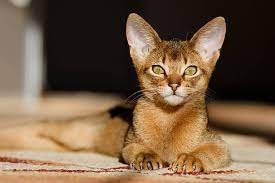
\includegraphics{src/abyssinian.jpeg}
    \caption{Abyssinian.}
    \label{fig:abyssinian}
\end{figure}

\subsection{Reference}
List and cite the references according to the style shown in
\cite{NIPS2012_c399862d}.
\section{Caution}
\subsection{Student number}
The student number corresponds to the individual identification code and does not need to be included in the dissertation. Please note that if you do, there is a risk of leaking personal information in the future.

\subsection{Thesis committee}
In the case of other research institutes, the Thesis committee is described as follows, for example.XXX \\
XXX \\
(Affiliate Professor Division of Information Science, Director R&D Development Center YYY Inc.) \\
XXX XXX \\
(Affiliate Professor Division of Information Science, Professor Graduate School of ZZZ ZZZ University) \\
XXX XXX \\
(Director, R&D Development Center, YYY Inc.)


\clearpage
\section*{Acknowledgements}
\addcontentsline{toc}{section}{Acknowledgements}%
Thank you

\clearpage
\bibliographystyle{ieeetr}
% Citation style is not specified in the format given by NAIST.
% Change the bibliography style following your specialization's conventions.
% See also: https://www.overleaf.com/learn/latex/Bibtex_bibliography_styles
% For NLP, you may want to use ACL's format; in that case,
% download acl.bst and add it to the project directory,
% and specify the bst file name in \bibliographystyle{}.

\bibliography{reference}
\clearpage

\appendix
\section*{Appendices}
\addcontentsline{toc}{section}{Appendices}%

\renewcommand*{\thesubsection}{\Alph{subsection}}
\subsection{Appendix-1}
This is an appendix. This is an appendix. This is an appendix. This is an appendix. This is an appendix. This is an appendix. This is an appendix. This is an appendix. This is an appendix. This is an appendix. This is an appendix. This is an appendix.
\subsection{Appendix-2}
This is an appendix. This is an appendix. This is an appendix. This is an appendix. This is an appendix. This is an appendix. This is an appendix. This is an appendix. This is an appendix. This is an appendix. This is an appendix. This is an appendix.

\end{document}
